\let\lesson\undefined
\newcommand{\lesson}{\phantomlesson{Bài 5: Mô hình động học phân tử chất khí}}
\chapter[Mô hình động học phân tử chất khí]{Mô hình động học phân tử chất khí}
\section{Lý thuyết}
\subsection{Chuyển động Brown}
\begin{center}
	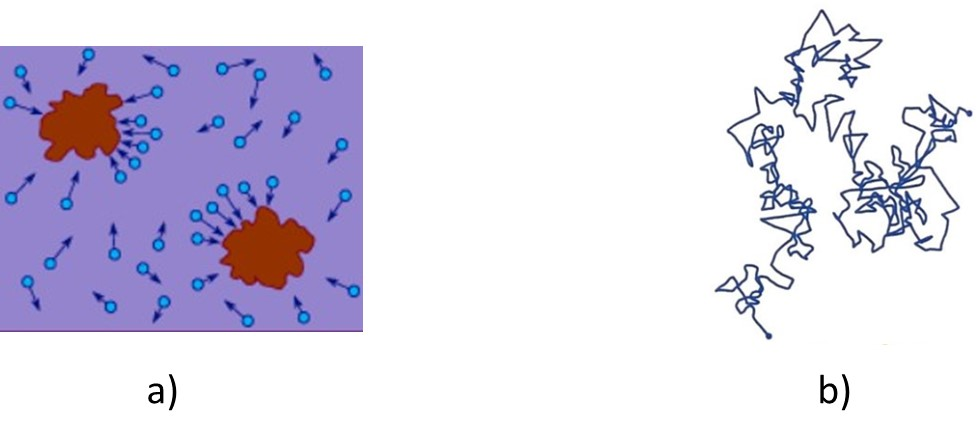
\includegraphics[width=0.5\linewidth]{../figs/VN12-Y24-PH-SYL-009-1}
	\captionof{figure}{a) Va chạm của các phân tử nước lên hạt phấn hoa, b) Minh hoạ quỹ đạo gấp khúc của một hạt phấn hoa trong nước. }
\end{center}
Chuyển động Brown là chuyển động hỗn loạn không ngừng, không theo quy luật, có quỹ đạo là những đường gấp khúc bất kì của các hạt nhẹ trong chất lỏng và chất khí. Chuyển động Brown chứng tỏ các phân tử chất khí chuyển động hỗn loạn, không ngừng. Nhiệt độ càng cao, các phân tử chuyển động càng nhanh.
\subsection{Chất khí}
\subsubsection{Tính chất của chất khí}
Chất khí có một số tính chất sau:
\begin{itemize}
	\item Chất khí có hình dạng và thể tích của vật chứa nó.
	\item Chất khí có khối lượng riêng nhỏ hơn nhiều so với chất lỏng và chất rắn.
	\item Chất khí dễ bị nén.
	\item Chất khí gây ra áp suất lên thành bình chứa nó. Khi nhiệt độ tăng, áp suất khí tác dụng lên thành bình tăng.
\end{itemize}
\subsubsection{Lượng chất}
Mol là lượng chất trong đó chứa số phân tử (hoặc nguyên tử) bằng 
$$N_A\approx\SI{6.02E23}{\mole^{-1}}$$
$N_A$ được gọi là số Avogadro (số phân tử trong 1 mol chất).\\
Khối lượng mol của một chất là khối lượng của $\SI{1}{\mole}$ chất đó, được kí hiệu là $M$.\\
Nếu một mẫu chất có khối lượng $m$, chứa $N$ phân tử thì số mol $n$ của mẫu chất đó được xác định:
$$n=\dfrac{N}{N_A}=\dfrac{m}{M}.$$
\subsection{Mô hình động học phân tử chất khí}
Nội dung mô hình động học phân tử chất khí gồm các ý chính như sau:
\begin{itemize}
	\item Chất khí gồm tập hợp rất nhiều các phân tử có kích thước rất nhỏ so với khoảng cách trung bình giữa chúng.
	\item Các phân tử khí luôn chuyển động hỗn loạn, không ngừng và được gọi là chuyển động nhiệt. Nhiệt độ càng cao, các phân tử khí chuyển động càng nhanh.
	\item Trong quá trình chuyển động, các phân tử khí va chạm với thành bình chứa, gây ra áp suất lên thành bình.
\end{itemize}
\begin{center}
	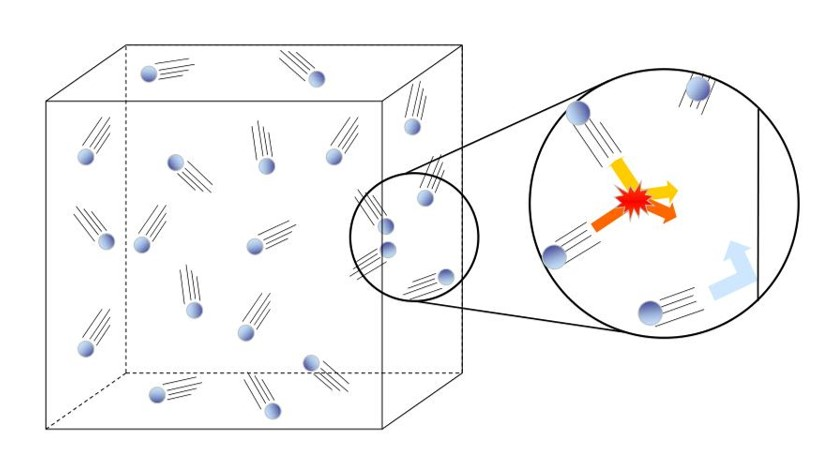
\includegraphics[width=0.4\linewidth]{../figs/VN12-Y24-PH-SYL-009-2}
	\captionof{figure}{Các phân tử va chạm vào nhau và va chạm vào thành bình trong quá trình chuyển động nhiệt.}
\end{center}
\subsection{Khí lí tưởng}
Khí lí tưởng có các đặc điểm sau:
\begin{enumerate}[label=\arabic*.]
	\item Các phân tử khí được coi là các \textit{chất điểm}, không tương tác với nhau khi chưa va chạm.
	\item Các phân tử khí tương tác khi va chạm với nhau và va chạm với thành bình. Các va chạm này là va chạm \textit{hoàn toàn đàn hồi}.
\end{enumerate}
\luuy{Mô hình khí lí tưởng đơn giản hơn khí thực (khí tồn tại trong thực tế) nhưng vẫn phản ánh được các đặc điểm cơ bản của khí này.}
\section{Mục tiêu bài học - Ví dụ minh hoạ}
\begin{dang}{Phân tích mô hình Brown, nêu được các phân tử trong chất khí chuyển động hỗn loạn.}
	\viduii{2}
	{Khi quan sát tia nắng mặt trời chiếu qua cửa sổ vào trong phòng, ta có thể thấy các hạt bụi trong ánh nắng chuyển động không ngừng. Chuyển động này có phải là chuyển động Brown không? Tại sao?
	
}
{\hide{Chuyển động của các hạt bụi trong trường hợp này không thể coi là chuyển động Brown vì chuyển động chủ yếu của các hạt bụi lúc bấy giờ là chuyển động theo dòng khí do hiện tượng đối lưu.
}
}
\end{dang}
\begin{dang}{Vận dụng được thuyết động học phân tử chất khí}
	\viduii{2}
	{Trong quá trình bơm xe đạp, khi lốp xe đã gần căng, càng về cuối của mỗi lần bơm thì ta càng thấy khó nén piston xuống. Hãy giải thích hiện tượng trên.
	
}
{\hide{Càng về cuối quá trình bơm săm xe đạp, săm xe đã căng và khó tăng thể tích chứa khí bên trong. Trong khi đó, sau mỗi lần bơm thì số phân tử khí bên trong săm tăng lên đáng kể và làm tăng mật độ phân tử khí bên trong. \\
	Theo thuyết động học phân tử chất khí, khi mật độ phân tử khí bên trong săm tăng thì số va chạm của các phân tử khí lên thành săm và piston tăng. Do đó, áp suất khí tác động lên piston tăng và làm cho piston khó nén xuống hơn.
}
}

\viduii{2}
{Một phân tử oxygen đang chuyển động qua tâm một bình cầu có đường kính $\SI{0.20}{\meter}$. Tốc độ của phân tử là $\SI{400}{\meter/\second}$. Ước tính số lần phân tử này va chạm vào thành bình chứa trong mỗi giây. Coi rằng tốc độ của phân tử là không đổi.
}
{\hide{Trong điều kiện lý tưởng, xem như phân tử oxygen chuyển động thẳng và không bị đổi hướng do va chạm với các phân tử khí khác, tốc độ của phân tử là không đổi và va chạm của phân tử khí với thành bình là tuyệt đối đàn hồi. Ban đầu phân tử khí này chuyển động qua tâm bình cầu nên khi chạm vào thành bình, phân tử khí sẽ bật ngược trở lại với tốc độ như cũ và cũng đi qua tâm bình cầu.\\
Khoảng thời gian giữa 2 lần liên tiếp phân tử khí va chạm với thành bình:
$$T=\dfrac{2R}{v}=\dfrac{\SI{0.2}{\meter}}{\SI{400}{\meter/\second}}=\SI{5E-4}{\second}.$$
Số lần phân tử khí này va chạm vào thành bình trong mỗi giây:
$$f=\dfrac{1}{T}=2000.$$
}
}
	
\end{dang}